\section{Datasets}

\subsection*{Phoenix Crime Dataset}
This CSV file includes crime incidents from the city of Phoenix since November 1st, 2015. It holds Homicides, rapes, robberies, burglaries, thefts and more. It also includes the location of the crimes as ZIP code.
\begin{itemize}
	\item Source: https://www.phoenixopendata.com/dataset/crime-data
	\item Size: 28'397 KB
	\item Format: CSV
\end{itemize}
\begin{figure}[H]
    \centering
    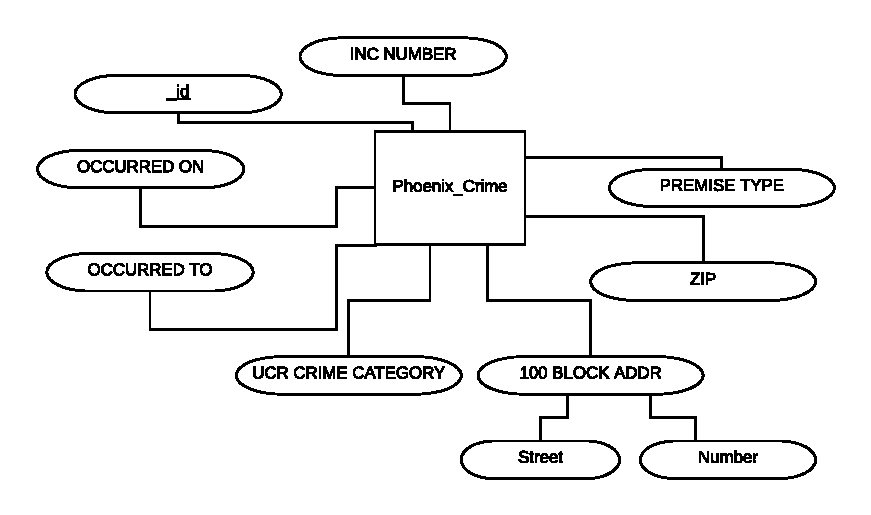
\includegraphics[width=1\textwidth]{g4-er-crime-dataset}
    \caption{ER-Diagram Phoenix Crime }
    \label{fig:phoenixCrime}
\end{figure}

\subsection*{Yelp Dataset}
The Yelp Dataset includes five different JSON files. For our analysis we only use the business and the review file. In the review file all the businesses are only listed with an ID. Therefore, we need the business file to cross reference it with the locations of these businesses. This dataset lists information about ten different cities including Phoenix.
We integrated these two datasets and separated the business from its address because we will create a separated address entity in our database.
\begin{itemize}
	\item Source: https://www.kaggle.com/yelp-dataset/yelp-dataset/download
	\item Filename: yelp\_academic\_dataset\_business.json
	\item Filename: yelp\_academic\_dataset\_review.json
	\item Size: business.json (135'039 KB), review.json (5'222'145 KB)
	\item Format: JSON
\end{itemize}
\begin{figure}[H]
    \centering
    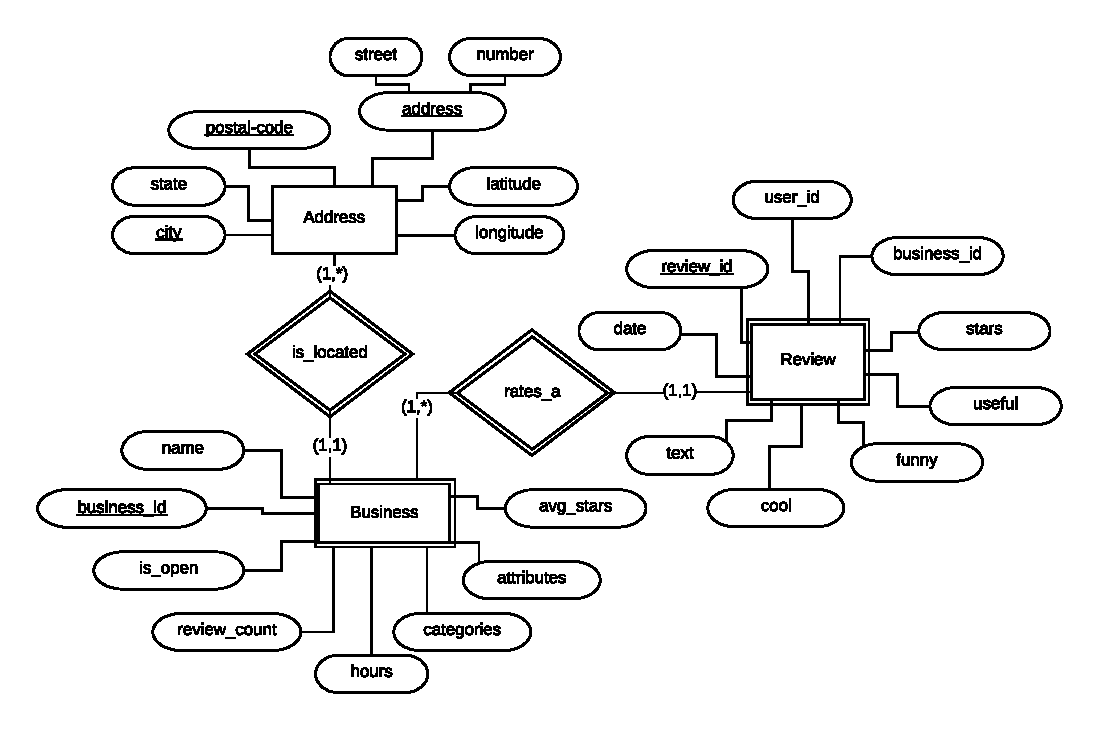
\includegraphics[width=1\textwidth]{g4-er-yelp-dataset}
    \caption{ER-Diagram Yelp}
    \label{fig:yelpER}
\end{figure}

\subsection*{Pain Pill in the USA Dataset}
The "pain pill in the USA" dataset holds information about the pain pill sales in the whole US. For our analysis we are only looking at the pain pill usage in Phoenix, AZ.
Unfortunately, this dataset only contains data until 2012. But we decided to use it anyway because it is a quite big dataset with interesting data and it allows us to compare it to the other two Datasets, if we ignore the different timespans.
\begin{itemize}
	\item https://www.kaggle.com/paultimothymooney/pain-pills-in-the-usa
	\item Size: 78'121'847 KB
	\item Format: TSV
\end{itemize}
\begin{figure}[H]
    \centering
    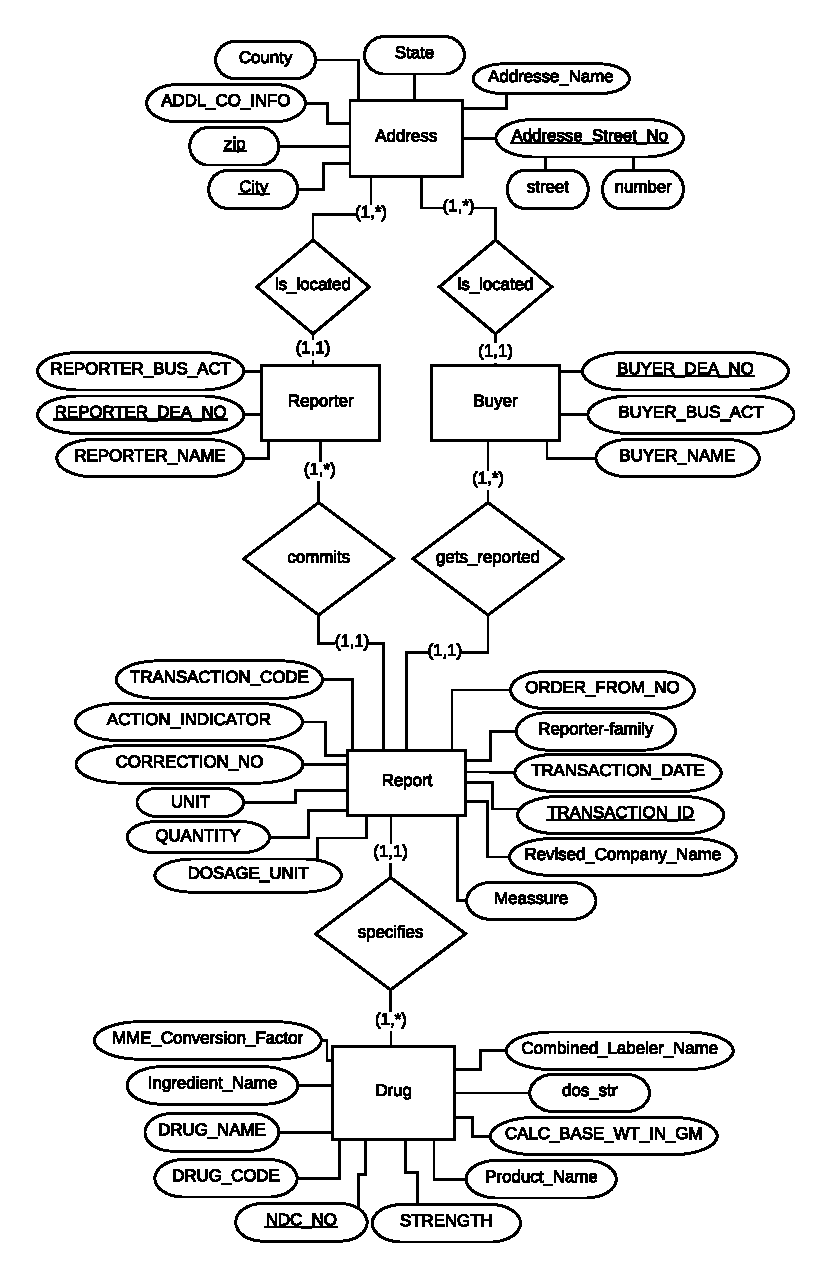
\includegraphics[width=1\textwidth]{g4-er-pain-pill}
    \caption{ER-Diagram Pain Pill Usage in the US}
    \label{fig:pillER}
\end{figure}

\subsection*{Integrated Entity Relation Diagram}
During the integration process we had to adapt our integrated entity relation diagram.
We realized that we had made a mistake in our integrated Entity Relation Diagram.
By oversimplification the grouping of the information we lost significant information. Therefore, we had to work with triple relations.
\begin{figure}[H]
    \centering
        %\subfloat[CAPTION]{BILDERCODE}\qquad
        \subfloat[Excerpt integrated ER-Diagram Version 1\label{fig:ERLessonsLearndV1}]{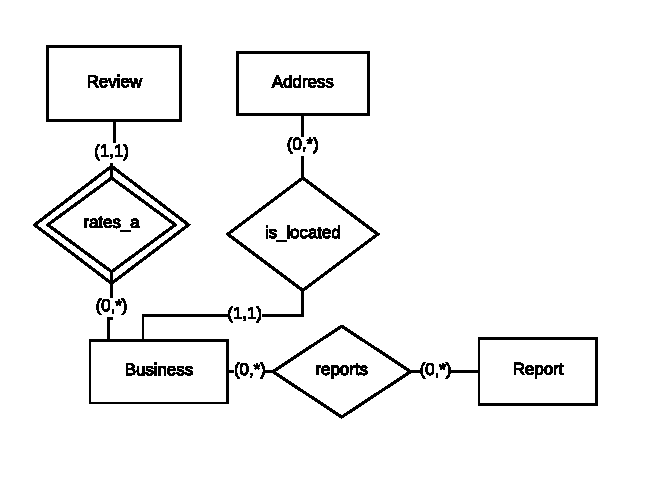
\includegraphics[width=0.45\textwidth]{g4-er-lessons-learnd-v1}}\qquad
        \subfloat[Excerpt integrated ER-Diagram Version 2\label{fig:ERLessonsLearndV2}]{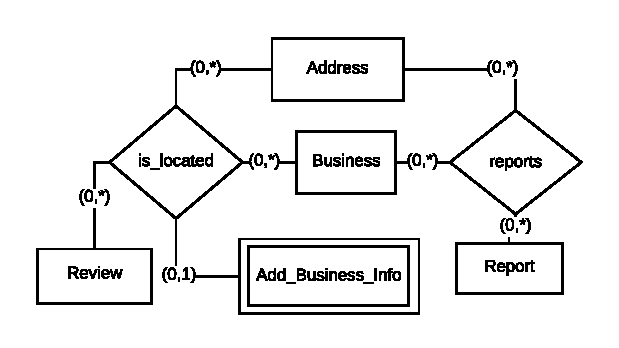
\includegraphics[width=0.45\textwidth]{g4-er-lessons-learnd-v2}}
    \caption{Excerpt from our ER-Diagrams}
    \label{fig:erv1v2}
\end{figure}
This Entity Relation works if we just want to compare different businesses. But in our case we are interested in the location of each Review and Report. With this integration we would have lost the information which business location belongs to which Report and Review.\\
We fixed that by working with 2 triple relation in our schema. One to tie a Review to a specific Business at an address and one which did the same for a Report of a drug purchase.\\
We tried to keep our tables address and business as small as possible without duplicated information. Because of that we have more information saved in the relations reports and is\_located. In reports we connected the address, business and the report and in is\_located the address, business, review and add additional\_business\_info.\\

\subsection*{Relational schema}
For presentation reasons, shortened add\_business\_info to add\_bus\_info.
\begin{center}
    \begin{tabbing}
        address \qquad\qquad\= (\uline{id}, zip, city, street, street\_number, county, state,\\
        \hspace{26mm} address\_name, longitude, latitude, addl\_co\_info)\\
        business \> (\uline{id}, business\_name, DEA\_no)\\
        crime \> (\uline{id}, inc\_number, premise\_type, occurred\_on,\\
        \hspace{26mm} occured\_to, ucr\_crime\_category)\\
        report \> (\uline{id}, transaction\_id, correction\_no, action\_indicator,\\
        \hspace{26mm} transaction\_code, order\_from\_no, reporter\_family,\\
        \hspace{26mm} transaction\_date, reviesed\_company\_name, measure, unit,\\
        \hspace{26mm}  quantity, dosage\_unit)\\
        drug \> (\uline{ndc\_no}, combined\_labeler\_name, dos\_str, \\
        \hspace{26mm} calc\_base\_wt\_in\_gm, product\_name, strength, drug\_code \\
        \hspace{26mm} drug\_name, ingredient\_name, mme\_conversion\_factor)\\
        is\_located \> (\uline{id}, \uwave{address\_id}, \uwave{business\_id}, reviewed\_business\_id)\\
        occured\_at \> (\uline{\uwave{address\_id}, \uwave{crime\_id}})\\
        specifies \> (\uline{\uwave{transaction\_id}, \uwave{ndc\_id}})\\
        reports \> (\uline{\uwave{transaction\_id}, \uwave{business\_id}, \uwave{address\_id}, role}, bus\_act)\\
        add\_bus\_info \> (\uline{\uwave{reviewed\_business\_id}}, is\_open, review\_count,\\ 
        \hspace{26mm} hours, categories, attributes, avg\_starts)\\
        review \> (\uline{review\_id}, \uwave{business\_id}, user\_id, date, text, cool, funny, useful, stars)\\
    \end{tabbing}    
\end{center}

\begin{figure}[H]
    \centering
    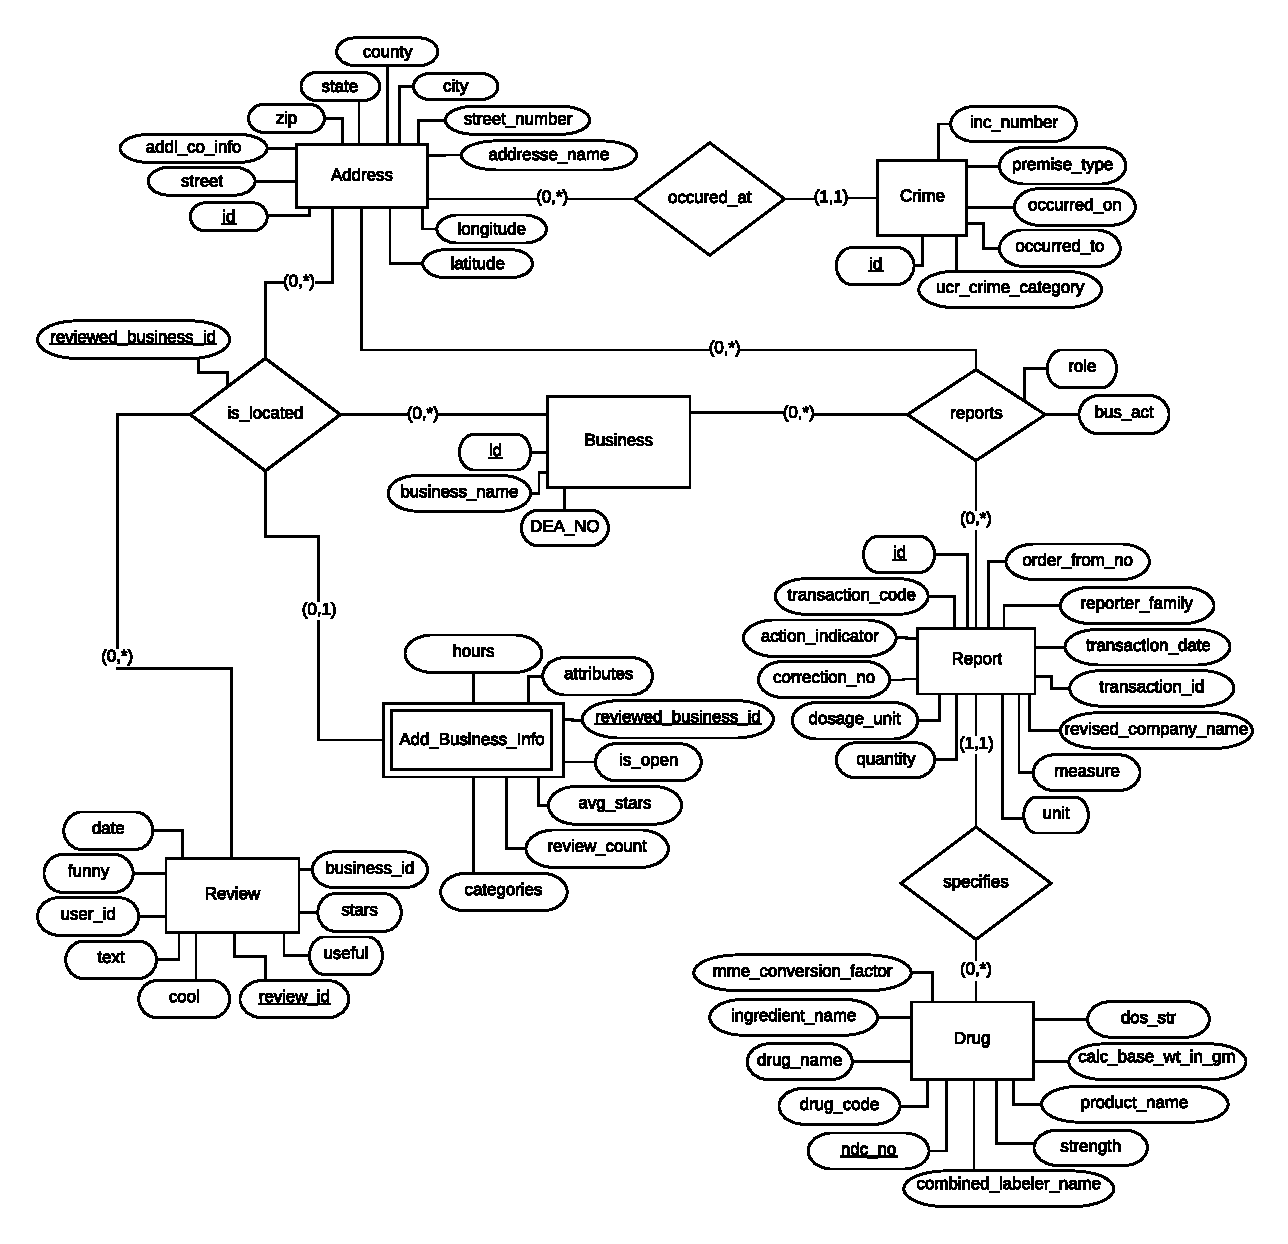
\includegraphics[width=1\textwidth]{g4-er-integrated}
    \caption{Integrated ER-Diagram}
    \label{fig:integratedER}
\end{figure}

\section{Data Integration}

The most significant part of this database project for us was the integration. We decided to us MySQL for this project because we already had some basic knowledge about it. To work and interact with the database we use Python. Before we could start to insert our data into the database we had to clean and prepare our initial datasets.

\subsection*{Initial findings}
First we integrated the Crime dataset because it is the smallest dataset and it seemed like a good idea to "start small". For the integration we parsed the CSV crime data and split the address. We independently created the primary key for the tables \textit{address} and \textit{crime} within Python. We looped through the CSV file and chunked the data for the insertion into the tables. Following that, we used the method executemany() to save time.\\
During the loop of the CSV, we saved the respective primary keys into a text file that belong together for the relation between \textit{crime} and \textit{address}. With the information text file we inserted the data into \textit{occured\_at}. After fixing some small issues this worked and we felt confident to start working on our biggest dataset.\\
But after trying we realized the same method would have taken multiple days to weeks for the Pain Pill dataset. Therefore, we had to obtain another solution.\\
Console log snippet:
\begin{lstlisting}
    time passed: 79.588
    executed 200000 rows from 178598027: 0.11%
\end{lstlisting}
\smallskip
We started all over again but this time with the Pill Dataset because it is by far the largest dataset with almost 80 GB. (Fun Fact: There are about 400 million reports in the Pill Dataset.)\\
The first change we made was to use an incremental approach. We processed the data and first inserted the tables \textit{business}, \textit{drug} and \textit{address} and added an auto-incremented primary key. After we looped through our dataset again to build the relations between these tables. We divided the addresses into files by postal code. Because of that it was possible to get the information to form the relations more quickly.\\
For the milestone p2, we integrated the entire database using beforehand described approaches. But shortly after submitting the integrated database we realized that we still have errors in our database. With our integration we lost important location information, and some of our foreign keys were not correctly linked. So we decided to integrate the whole database again and make some tweaks to our existing integration code.\\
For our final approach we proceeded as it follows in the next sections.

\subsection*{Data Processing}
Our goal was to compare the data geographically using postal codes. Therefore, we had to make sure to check all the postal codes. Unfortunately, there were data records, where the postal code was missing. If there were no postal codes, we would change it to 00000. This allowed us to use the postal code in combination with street, street\_number and state to find database entries before the primary key was added.\\
We split the address into street and street\_number. We decided to do so in order to have the possibility of structuring our evaluation not only by postal code but also by streets. The most common abbreviations rd\//rd. and st were changed to Road and Street to have uniformly street names.

\subsection*{MySQL settings}
Important MySQL Database settings we changed during the integration process.
\begin{lstlisting}[language=SQL]
    SET GLOBAL max_allowed_packet=1073741824 
\end{lstlisting}
We increased the communication packet size for a single SQL statement sent to the MySQL server.\footnote{\url{https://dev.mysql.com/doc/refman/8.0/en/packet-too-large.html}} In order to enlarge our chunk and send bigger statements to the server.
\begin{lstlisting}[language=SQL]
    SET GLOBAL innodb_buffer_pool_size=12884895290 
\end{lstlisting}
The innodb\_buffer\_ pool\_size specifies the amount of memory allocated to the MySQL InnoDB buffer pool. By increasing the size, the operation is performed in chunks. \footnote{\url{https://dev.mysql.com/doc/refman/8.0/en/innodb-buffer-pool-resize.html}}
\begin{lstlisting}[language=SQL]
    SET autocommit = 0
\end{lstlisting}
With autocommit MySQL starts the session for each new connection and does a commit after each SQL statement. If autocommit is disabled the session has always an open transaction. A transaction is ended by a commit or a rollback statement. \footnote{\url{https://dev.mysql.com/doc/refman/8.0/en/innodb-autocommit-commit-rollback.html}}
\begin{lstlisting}[language=SQL]
    SET GLOBAL local_infile = true
\end{lstlisting}
With the option local\_infile it is possible to insert a file directly into a table. Which is a lot faster than inserting each row by its own or even using executemany(). \footnote{\url{https://dev.mysql.com/doc/refman/8.0/en/load-data.html}}

\subsection*{Data insertion}
After creating the schema and the respective tables, we started by inserting the data for the empty entity tables, ignoring the relations between them at first.\\
If a table already had data from a previous insert, we would proceed as followed. We used this SQL statement to gather all the information needed to check if for example a specific address exists already in the respective table or not.
\begin{lstlisting}[language=SQL]
    SELECT street, street_number, zip, state, id 
    FROM Address where state='AZ';
\end{lstlisting}
We also used this kind of statement to get all the information needed for the relations between the tables.\\
But not all tables were complex to integrate. Tables containing information from only one dataset could be inserted easily, in contrast to for example the \textit(address) table which had data from multiple datasets.

\subsection*{Overall data handling}
We ended up inserting the datasets in the following order:
\begin{itemize}
    \item Pain Pill usage in the US
    \item Phoenix Crime
    \item Yelp
\end{itemize}
In the end we decided it was easier to have multiple Python files for each set. To separate different steps like data processing, insertion and table adjustments. It also made our troubleshooting easier.\\
Rough overview over the final process of data integration:
\begin{itemize}
    \item Pain Pill usage in the US
    \begin{itemize}
        \item[-] serializer
        \item[] It takes the TSV file, parses and divides the information to objects and saves them in one PKL file.
        \item[-] splitter
        \item[] It splits the PKL file into smaller, memory sized files, separated by postal code.
        \item[-] filter
        \item[] It deletes all duplicates so that there are no duplicated names or addresses in the database.
        \item[-] inserter
        \item[] The inserter finally inserts the data into the tables \textit{business}, \textit{address} and \textit{drug}.
        \item[-] report\_inserter
        \item[] Inserts \textit{report} and all relations between the tables. It loops through the CSV file and with the dea\_no and business\_name respectively zip, street, street\_no and state it selects the id from the corresponding table in the database.
    \end{itemize}
    \item Phoenix Crime
    \begin{itemize}
        \item[-] crime\_serializer\_filter
        \item[]  It takes the CSV file, parses the information, deletes duplicates and divides it into objects, which are saved in a PKL file.
        \item[-] crime\_address
        \item[] Inserts the data into \textit{address}, \textit{crime} and populates the relation between the two \textit{occured\_at} with the correct data. 
    \end{itemize}
    \item Yelp
    \begin{itemize}
        \item[-] yelp\_filter
        \item[] Parses the JSON file, deletes duplicates and divides it into objects, which are saved as PKL file.
        \item[-] yelp\_address
        \item[] Inserts the data into \textit{address}.  
        \item[-] yelp\_business
        \item[] Inserts the data into \textit{business}.  
        \item[-] yelp\_review
        \item[] Inserts the data into \textit{review}.  
        \item[-] yelp\_is\_located
        \item[] Inserts the data into \textit{is\_located}. 
        \item[-] yelp\_add\_info\_business
        \item[] Inserts the data into \textit{add\_info\_business}.   
    \end{itemize}
\end{itemize}

\section{Analysis and Visualization}

\subsection*{Analysis Goal}
As a reminder our research questing:
\begin{center}
    \textbf{\emph{Are there correlations between Yelp reviews, pain pill usage and crime rate in Phoenix, Arizona Us.}}
\end{center}
Our analysis goal was to figure out if there are correlations between Yelp reviews, the pain pill sales and the crime rate in Phoenix using the postal codes to split the city geographically. 

\subsection*{Undetected Error}
Unfortunately, our analysis did not start as planned. We had quite some problems with the SQL query analysing the pill sales in Phoenix, in contrast to the other two. All queries regarding the pill sales toke ages to finish and we started wondering, wether there is a problem or not.\\
After fixing a small query mistake, it turned out that we only got information from four different postal codes, as you can see here: \ref{fig:pillError}. Something was not be correct.
\begin{figure}[H]
    \centering
    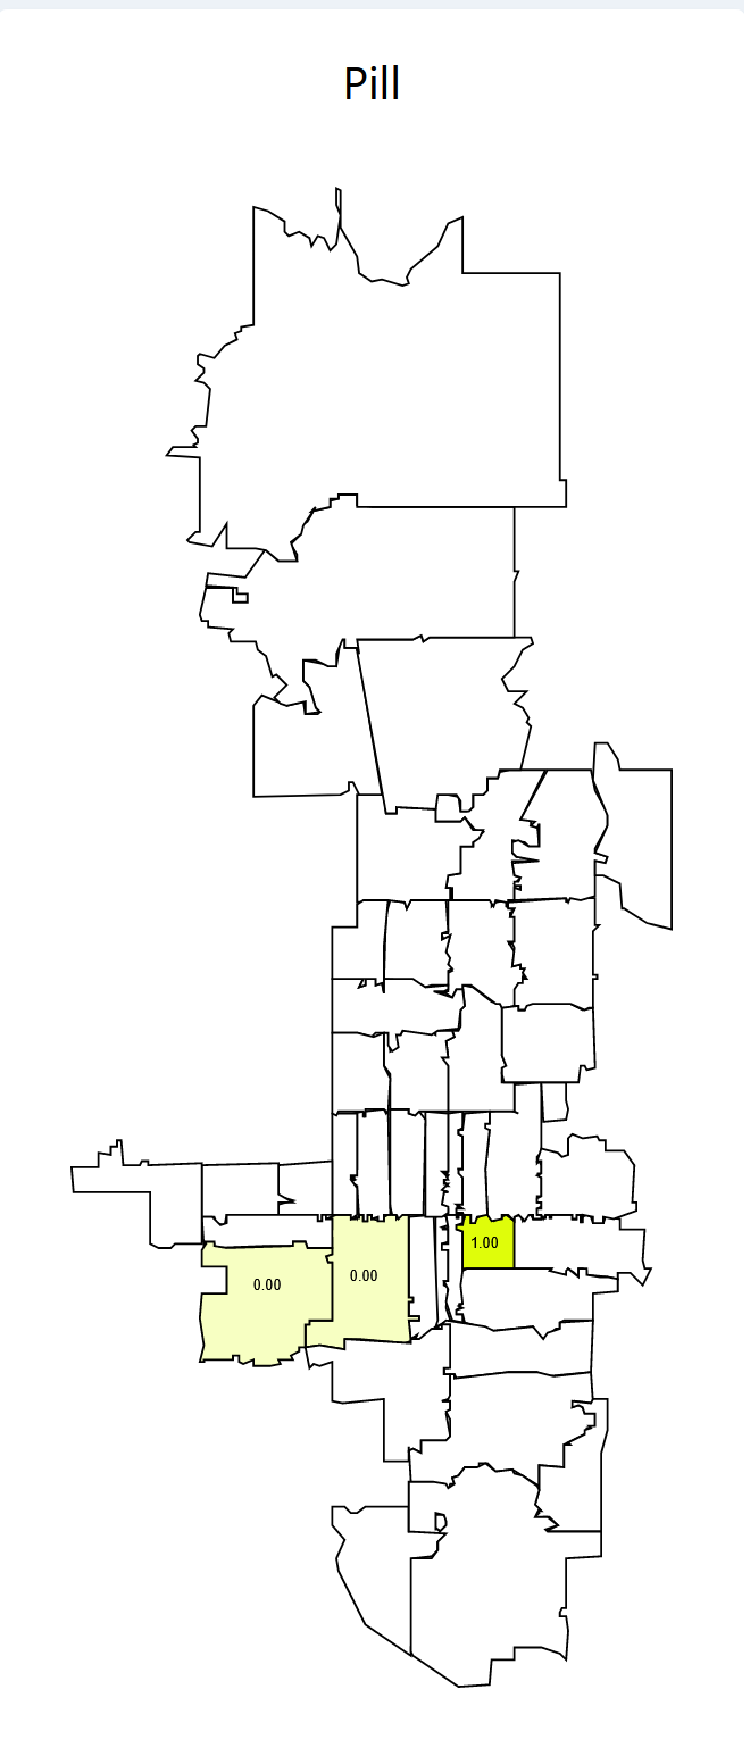
\includegraphics[width=0.25\textwidth]{g4-pill-error}
    \caption{Map showing only four different postal codes with pill sells}
    \label{fig:pillError}
\end{figure}
We got the Pain Pill Dataset from kaggle.com, but we found out that it was originally from the Washington Post. It is possible to download only a small part of the entire dataset.
\begin{itemize}
	\item https://www.washingtonpost.com/graphics/2019/investigations/dea-pain-pill-database/
	\item Size: 1'013'747 KB
	\item Format: TSV
\end{itemize}
We checked our database with some random data from the dataset. The tables themselves looked good, and we enclosed the issue to the relation \textit{reports}. \\
We decided not to integrate the whole \textit{reports} relation again. It holds about 400 million entries and takes about two days to integrate. And we did not know how long it would take to even find our mistake. Therefore, we decided to only add the fix the information from Phoenix. This allowed us to perform the complete analysis.\\
Nevertheless, we wanted to find the mistake we made in the relation \textit{reports}. In the pill dataset was one buyer and one reporter on each row. In the relation reports we defined whether it is a buyer or a reporter. This is where the mistake occurred. We linked the buyer and the reporter to the same address. We used the same column from the TSV file twice. We tested the relation, but unfortunately we did not notice this error.


\subsection*{SQL Queries}
In order to answer our research question we first had to evaluate each topic area by its own.
\subsection*{Crime}
We used the following SQL statement to count how many crimes were in each postal code section committed. We only selected crimes within the city of Phoenix without agglomeration.
\begin{lstlisting}[language=SQL]
    SELECT zip, count(*) FROM address 
    INNER JOIN (occurred_at 
    INNER JOIN crime ON occurred_at.crime_id = crime.id) 
    ON address.id = occurred_at.address_id 
    WHERE address.zip LIKE '850%'
    GROUP BY zip 
    ORDER BY zip;
\end{lstlisting}
We did not know whetter this data alone was meaningful enough. So we decided to also have a look at the population in the different areas. After we had tested it, we noticed that it did not influence the outcome much. So we decided not to use the population as a factor.

\subsection*{Review}
At the beginning we just got the average from the avg\_stars for each postal code. But we realized that might not be enough data because we do not know how many reviews were made in each postal code region.
\begin{lstlisting}[language=SQL]
    SELECT address.zip, CAST( AVG(avg_stars) AS FLOAT) 
    FROM address INNER JOIN 
    (is_located INNER JOIN add_business_info 
    ON is_located.reviewed_business_id 
    = add_business_info.reviewed_business_id) 
    ON address.id = is_located.address_id 
    WHERE address.state = 'AZ' 
    && address.city = 'Phoenix' 
    && address.zip LIKE '850%' 
    GROUP BY zip 
    ORDER BY zip;
\end{lstlisting}
Therefore, we changed our SQL statement and also looked at the number of reviews within a postal code region. We introduced a minimum of reviews needed to work with it. We tested various minimum review information and ended up using a minimum of 15. We belive it is better not to have any data than not meaningful enough data.
\begin{lstlisting}[language=SQL]
    SELECT address.zip, count(*), 
    CAST( AVG(avg_stars) AS FLOAT) 
    FROM address INNER JOIN 
    (is_located INNER JOIN add_business_info 
    ON is_located.reviewed_business_id 
    = add_business_info.reviewed_business_id) 
    ON address.id = is_located.address_id 
    WHERE address.state = 'AZ' 
    && address.city = 'Phoenix' 
    && address.zip LIKE '850%'
    GROUP BY zip 
    ORDER BY zip;
\end{lstlisting}

\subsection*{Pain Pill}
Similarly, we gathered the information for the Pain Pill sales. We calculated quantity times dosage\_unit and added it up for each postal code.
\begin{lstlisting}[language=SQL]
    SELECT zip, quantity, dosage_unit 
    FROM address INNER JOIN 
    (reports INNER JOIN report 
    ON reports.transaction_id = report.id) 
    ON address.id = reports.address_id 
    WHERE address.state = 'AZ' 
    && address.city = 'Phoenix' 
    && address.zip LIKE '850%'
    ORDER BY zip;
\end{lstlisting}
Important to mention is that we only know were the Pain Pill was sold and not by whom it was bought. The buyer we mentioned before is the pharmacy which purchased the pills.

\subsection*{Visualization}
We visualized our analysis with a heat map. The heat map shows Phoenix (Arizona US) geographically divided by postal codes. 
\begin{figure}[H]
    \centering
    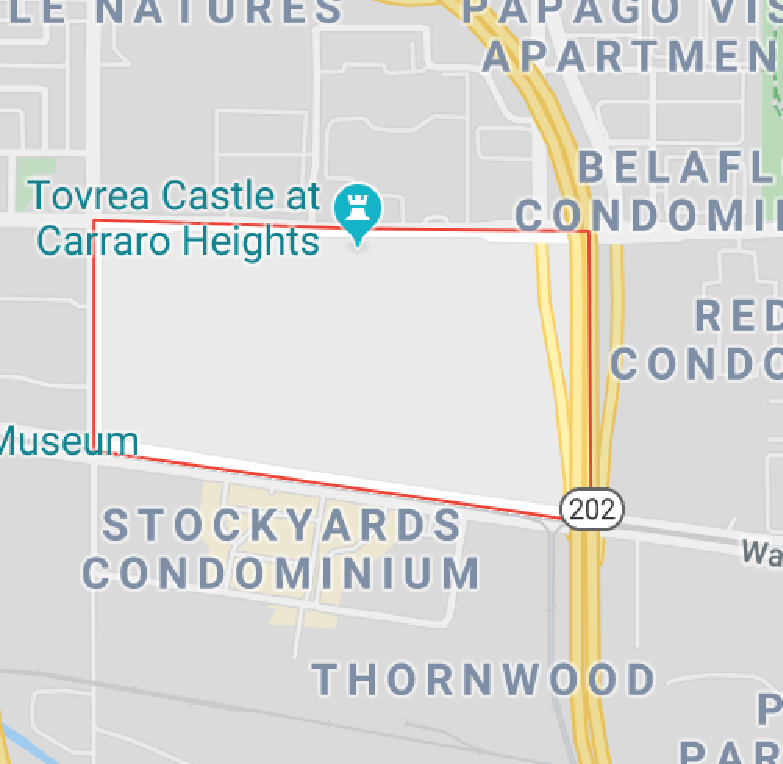
\includegraphics[width=0.3\textwidth]{g4-small-zip}
    \caption{Small postal code areas}
    \label{fig:zipArea}
\end{figure}
There are very small postal code areas in Phoenix. These are not represented in the heatmap. For example the Tovrea Castle \ref{fig:zipArea} has its own postal code. We had only little to non information concerning these small areas in our database. Therefore, we did not visualize them on our heat map.\\
We created the heatmaps through interactive SVG graphics in a Vue.Js web application. We could repurpose the areas of pheonix from AZ HomeTownLocator.\footnote{\url{http://zipatlas.com/us/az/phoenix/zip-code-comparison/population-density.htm}} But we had to assign the correct postal codes to each area with Adobe Illustrator by ourself. Then we implemented them in a generic Phoenix heat map component we used for all our different components. The result can be found on our website:\\
\url{http://db-project-group-4.lengweiler.com}

\subsection*{Analysis}
To compare all the data, we got from the different topic areas we had to normalize our data. We rescaled our data to have values between 0 and 1. For crime this was the amount of crime, for review the average stars and for the pill the sales.
\[
x_{new}= 
\left[\frac{x-x_{min}}{x_{max}-x_{min}}\right]
\] 
This allowed us to compare the different values for one topic and show them on a heat map.\\\\
For the combination of two maps, respectively two values we calculated the similarity between them.
\[
x_{new}= 
(1-|x_{1}-x_{2}|) * 2 - 1
\] 
This maps the similarity of the two on the interval [-1, 1]. Where 1 means they are exactly equal (positive correlation) and -1, they are completely different (negative correlation).\\
To match our research question, we had to invert the values for the average review. This meant that the in average worst rated areas had the value 1 and vice versa.\\
For the final map, where we compared all the three topics, we decided to use the standard deviation to check for similarily.
\[
std= 
\sqrt{\frac{\sum_{i = 0}^{N}{x_{i} - \overline{x}}}{N-1}}
\]



\begin{figure}[H]
    \centering
        %\subfloat[CAPTION]{BILDERCODE}\qquad
        \subfloat[Crime\label{fig:crime}]{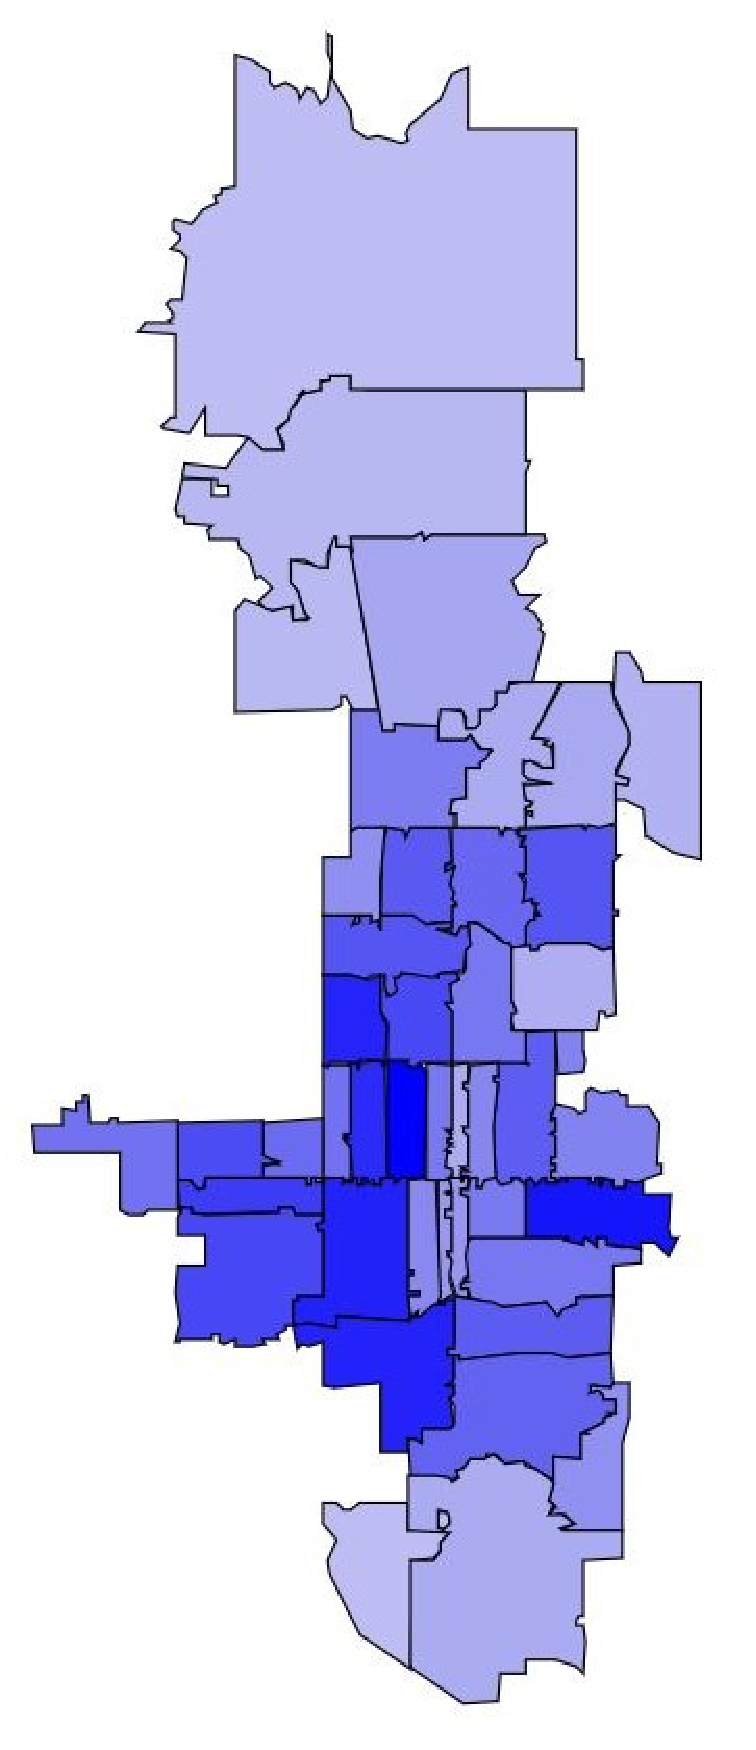
\includegraphics[width=0.2\textwidth]{g4-crime}}\qquad
        \subfloat[Review\label{fig:review}]{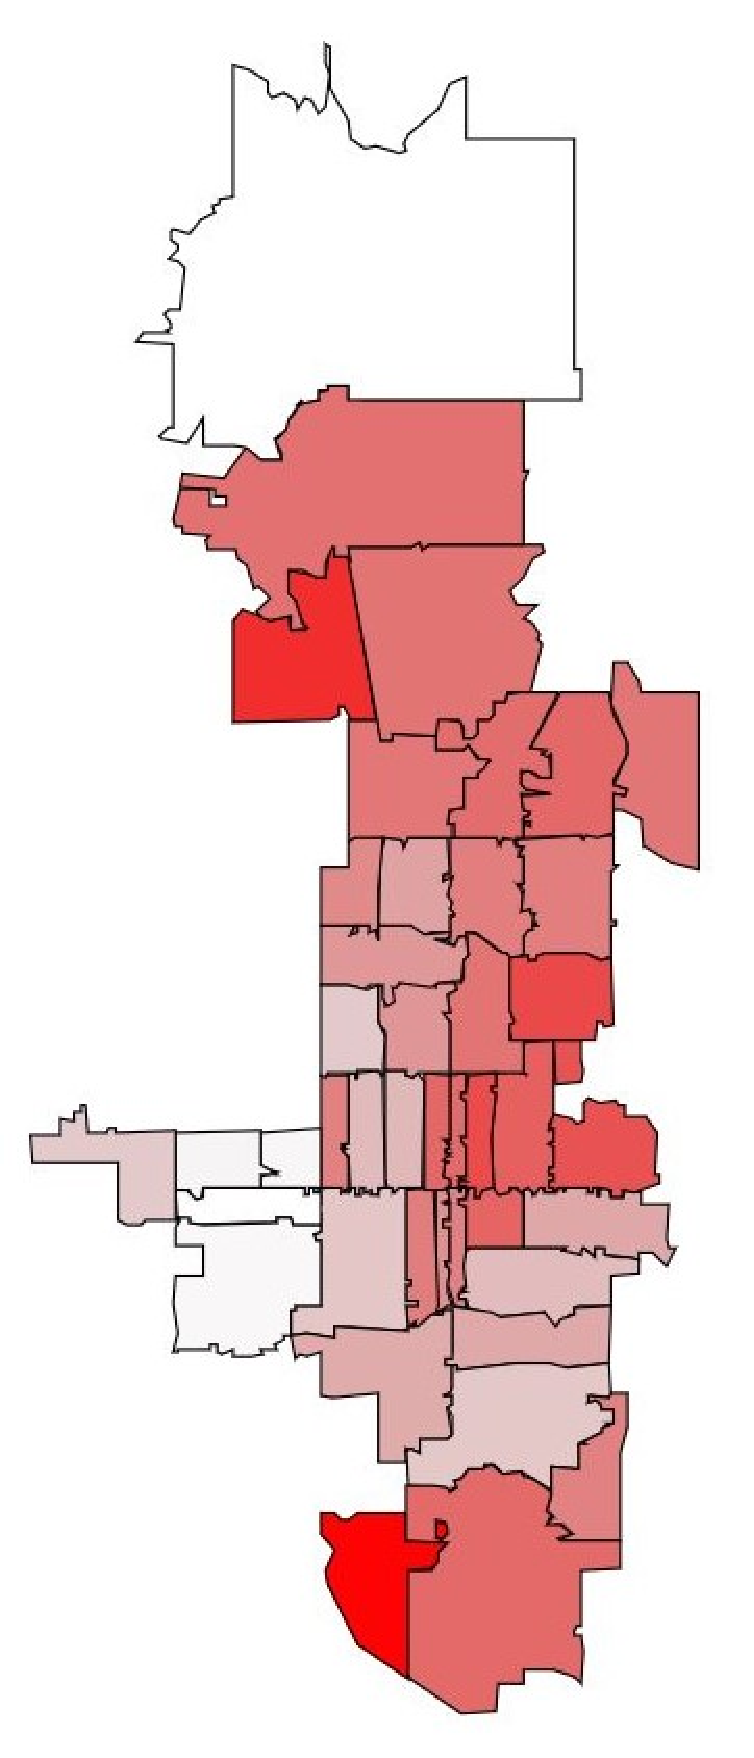
\includegraphics[width=0.2\textwidth]{g4-review}}
        \subfloat[Pain Pill\label{fig:pill}]{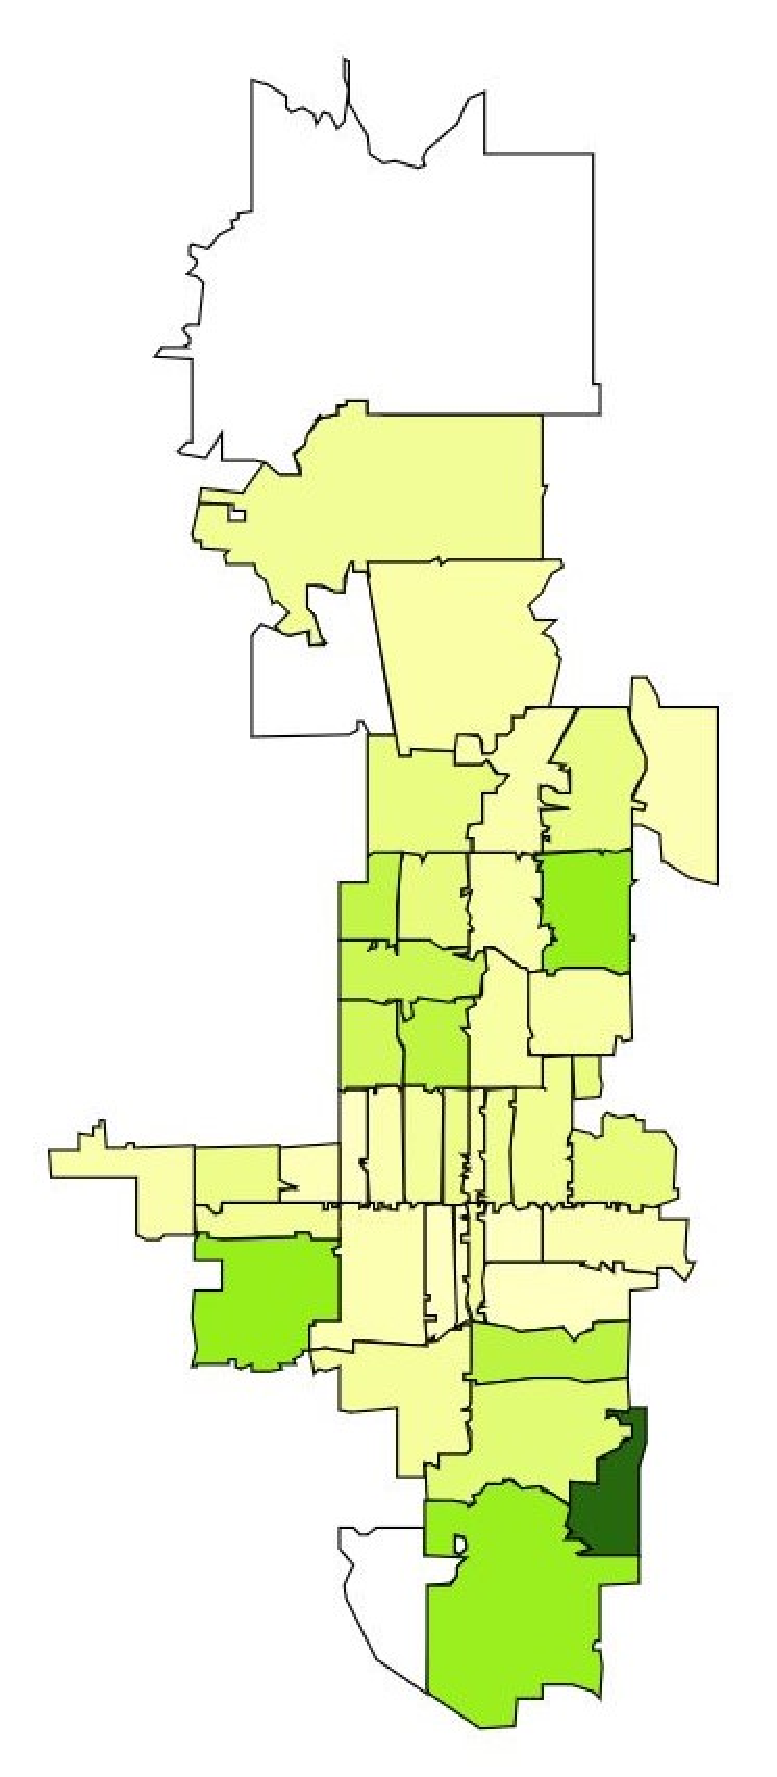
\includegraphics[width=0.2\textwidth]{g4-pill}}
    \caption{Analysed Heat Maps for each topic area}
    \label{fig:analysedSeperate}
\end{figure}
First, we looked at all the topic areas individually. The map \ref{fig:crime} shows the information about crime. The darker the color, the more incidents occurred in a postal code region. For the map \ref{fig:review} in the middle, it is the other way around. The darker the red the better was the average business ratings. Finally the Pain Pill map \ref{fig:pill}, the darker the green the more pills have been sold. We had no information in our database about the white postal code regions.
\begin{figure}[H]
    \centering
        %\subfloat[CAPTION]{BILDERCODE}\qquad
        \subfloat[Crime-Pill\label{fig:crimePill}]{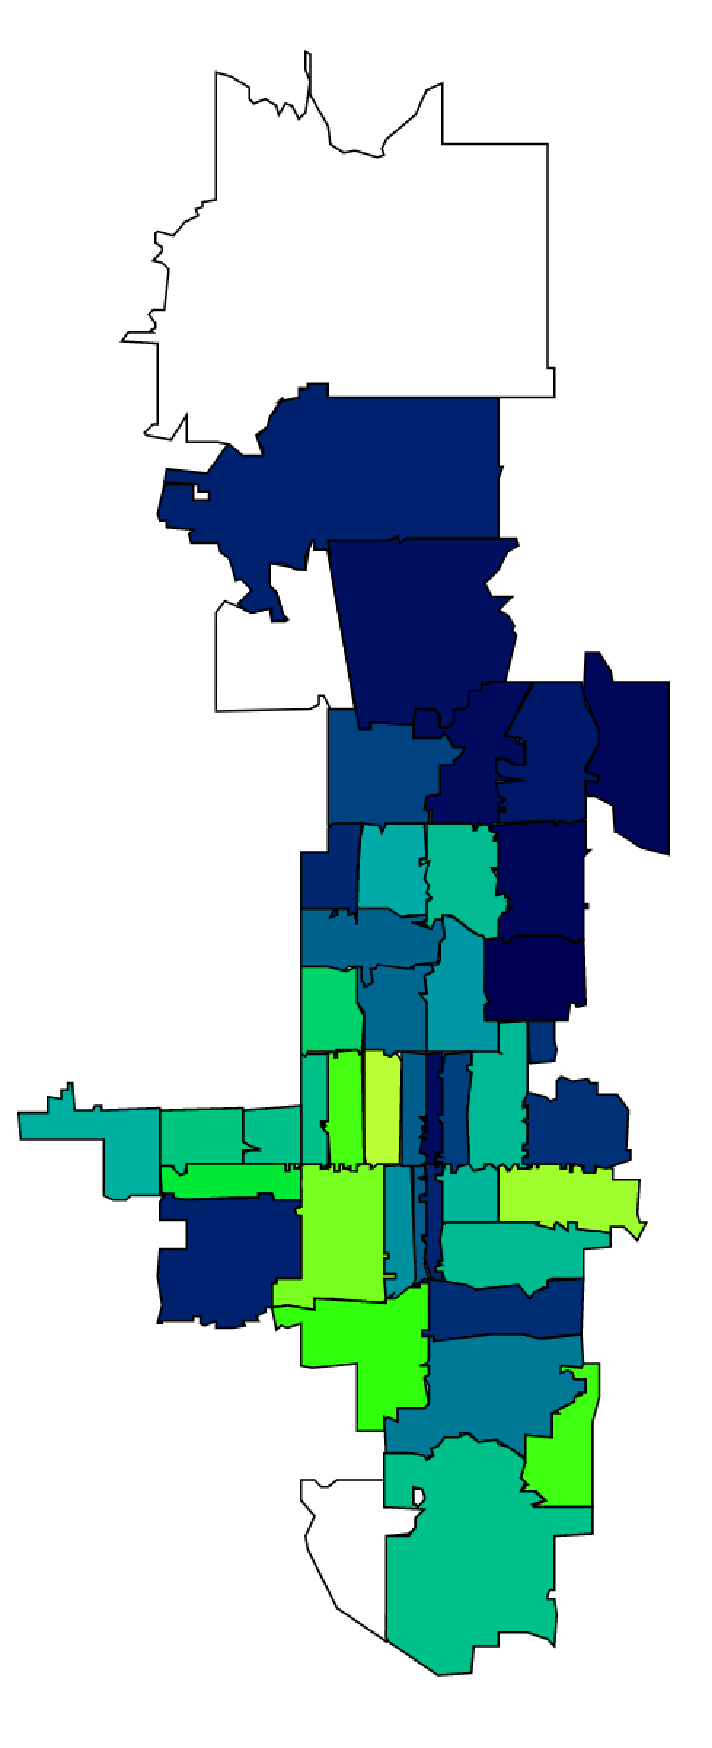
\includegraphics[width=0.2\textwidth]{g4-crime-pill}}\qquad
        \subfloat[Review-Crime\label{fig:reviewCrime}]{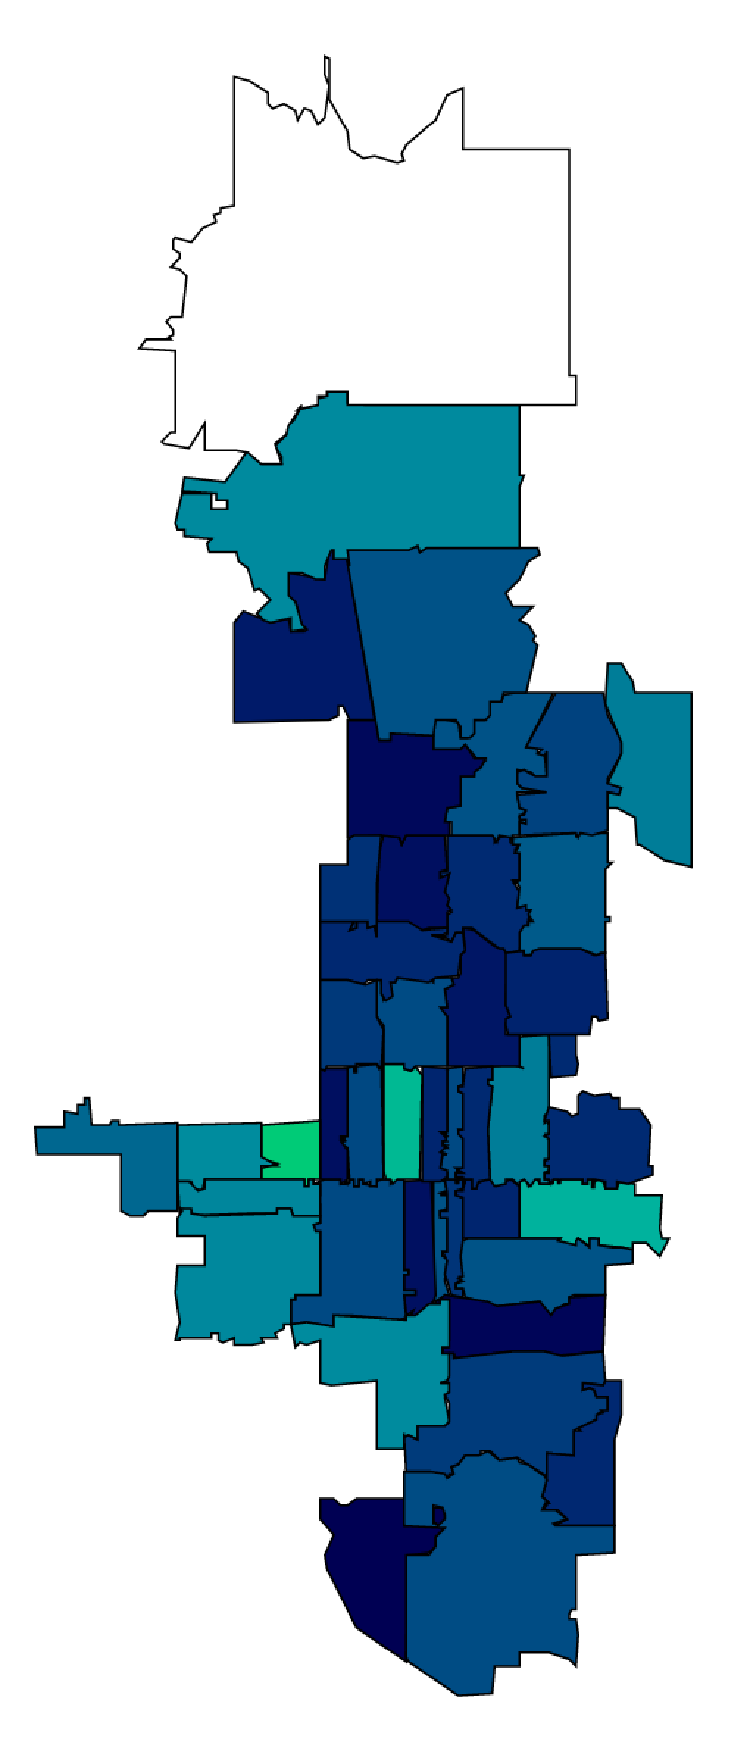
\includegraphics[width=0.2\textwidth]{g4-crime-review}}
        \subfloat[Review-Pill\label{fig:pillReview}]{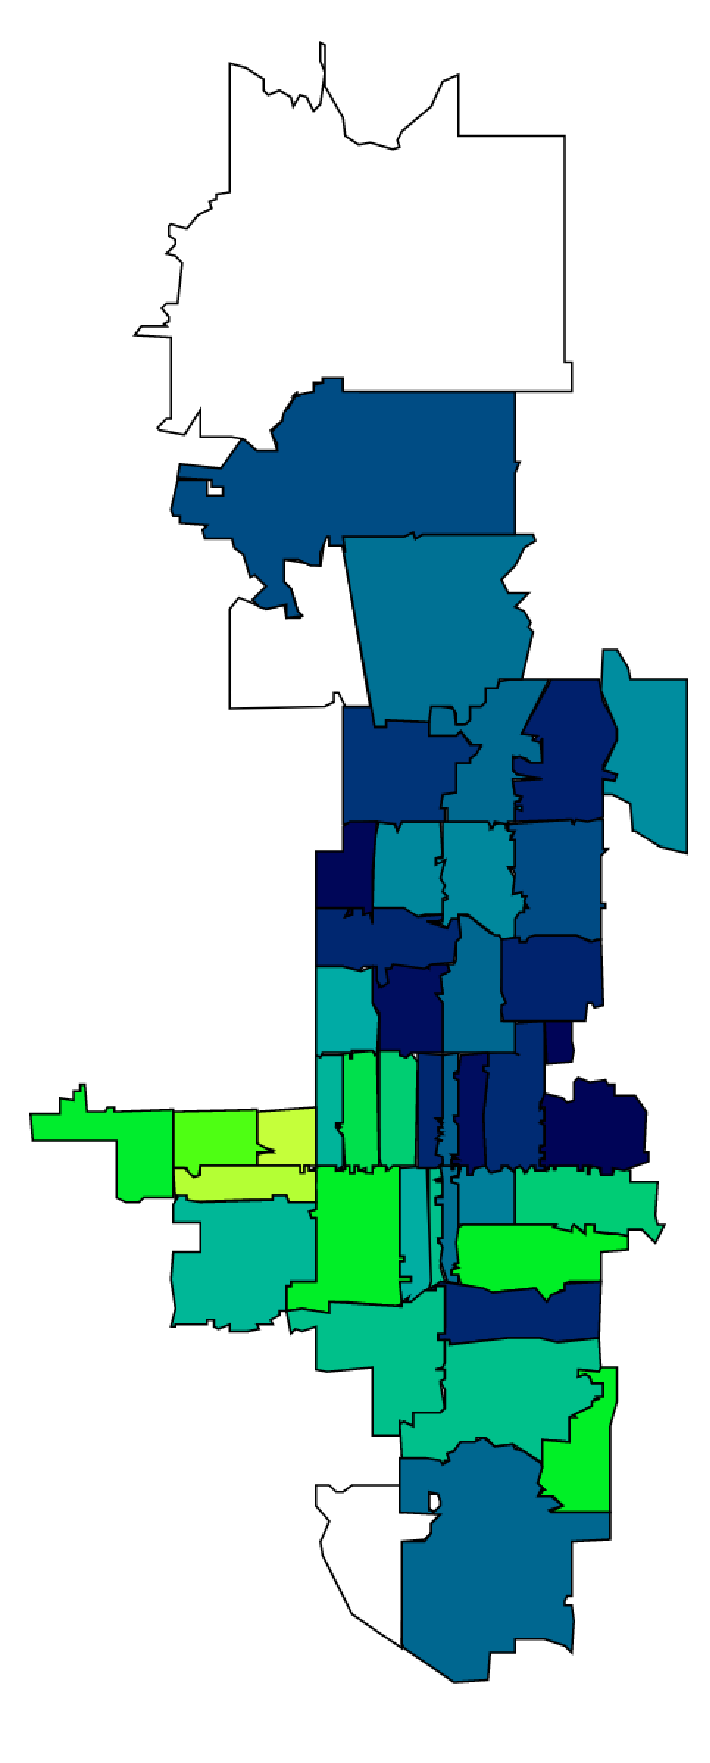
\includegraphics[width=0.2\textwidth]{g4-review-pill}}
    \caption{Analysed Heat Map for combined topic area}
    \label{fig:analysedCombinedTwoAreas}
\end{figure}
Next we linked two topic areas together to see if there were correlations between them. The darker the colors the higher the positive correlation and the lighter the color the higher the negative correlation. In order to compare the reviews with the other two topics we had to switch its values. Now the worst reviews are the highest values respectively the darkest color. It is clearly to see that there is a correlation between Reviews and Crime \ref{fig:reviewCrime}. In places where business ratings were low, the crime rate was higher and vice versa. This is the only correlation which is clearly visible. In the other maps are some correlations but not very pronounced.
\begin{figure}[H]
    \centering
    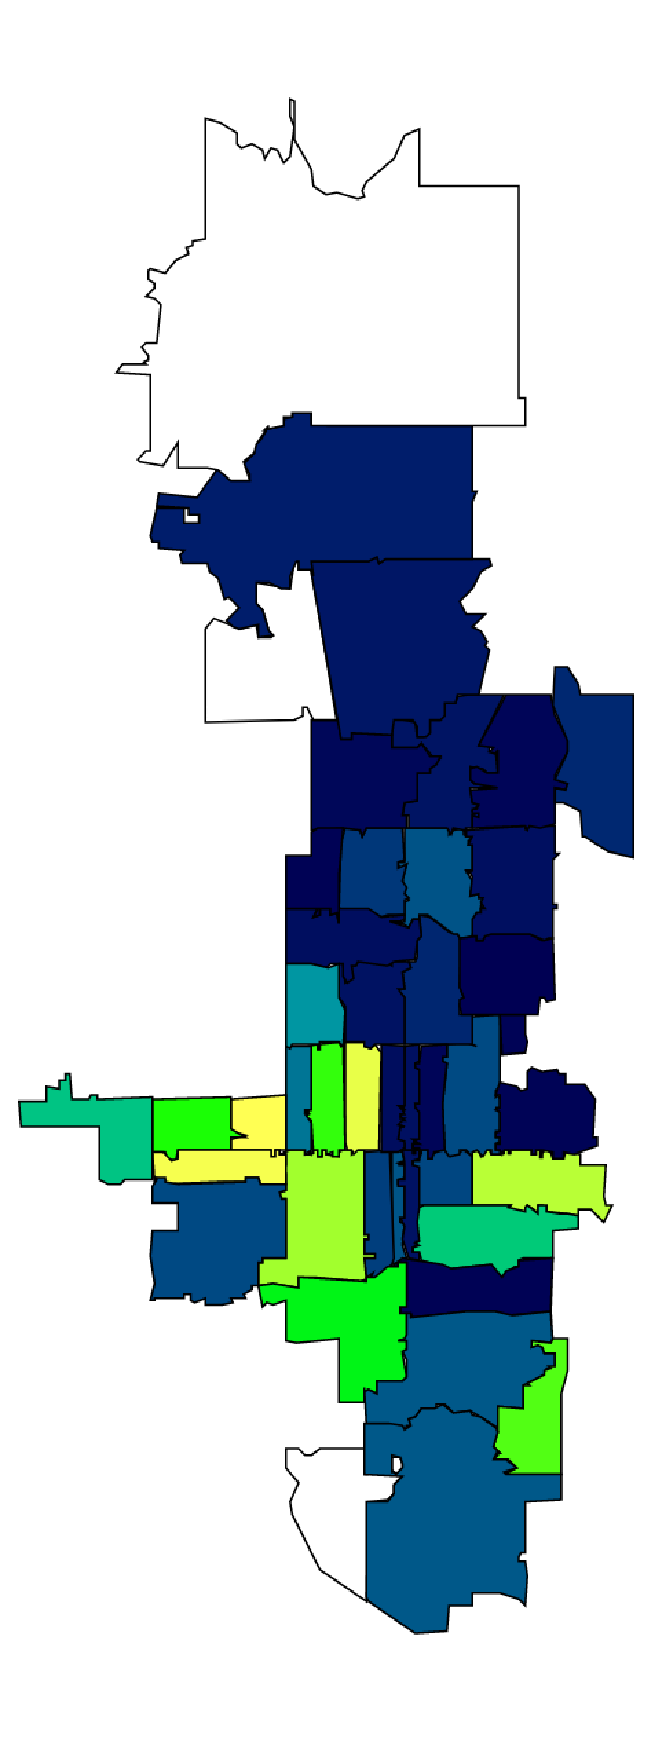
\includegraphics[width=0.25\textwidth]{g4-crime-pill-review}
    \caption{Analysed Heat Map combined all topic areas}
    \label{fig:crimePillReview}
\end{figure}
At the end we put together all three information. As you can see on the map \ref{fig:crimePillReview} the colors are pretty solid. That means between all three information Crime, Pain Pill and Review there is no strong correlation in our option.
\begin{center}
    \textbf{\emph{Are there correlations between Yelp reviews, pain pill usage and crime rate in Phoenix, Arizona Us.}}
\end{center}
Now we can answer this question. The only distinctly correlation we think is between the crime rate and the business reviews. With the others there are some overlaps but nothing explicit.
